% QiOpt4QNet manuscript for npj Quantum Information (Springer Nature template).
%
% Base text: the collaborator's draft. The penalty-calibration results,
% statistics and caveats have been rewritten from the artifacts in this
% repository (QNet_Sim/results/penalty_calibration/), so every calibration
% number below can be regenerated with the commands in QNet_Sim/results/README.md.
% Statements marked in supplementary.tex / the hand-over checklist as
% "not reproducible from this repository" come unchanged from the draft.
%
% Building needs the Springer Nature class (sn-jnl.cls), which is not in the
% repository, and the collaborator's figures in paper/figures/ (fig1, fig4-fig6).
% The two calibration figures are taken from QNet_Sim/results/penalty_calibration/figures/.
\documentclass[pdflatex,sn-nature]{sn-jnl}

\usepackage{graphicx}
\usepackage{multirow}
\usepackage{amsmath,amssymb,amsfonts}
\usepackage{amsthm}
\usepackage{booktabs}
\usepackage{array}
\usepackage{siunitx}
\usepackage{xcolor}
\usepackage{url}
\usepackage{enumitem}
\usepackage{microtype}
\usepackage{mathtools}

\graphicspath{{figures/}{../QNet_Sim/results/penalty_calibration/figures/}}
\sisetup{detect-all,group-separator={,},group-minimum-digits=4}
\newcommand{\E}{\mathbb{E}}
\newcommand{\Prb}{\mathbb{P}}
\newcommand{\Bset}{\mathcal{B}}
\newcommand{\Rset}{\mathcal{R}}
\newcommand{\Eset}{\mathcal{E}}
\newcommand{\Vset}{\mathcal{V}}
\newcommand{\eps}{\varepsilon}

\theoremstyle{plain}
\newtheorem{proposition}{Proposition}
\theoremstyle{remark}
\newtheorem{remark}{Remark}

\raggedbottom

\begin{document}

\title[Physics-aware entanglement orchestration]{Physics-aware entanglement orchestration in quantum networks: reliability-constrained routing and resource-specific QUBO calibration}

% --------------------------------------------------------------------------
% AUTHOR METADATA PLACEHOLDERS -- replace before submission.
% --------------------------------------------------------------------------
\author*[1]{\fnm{Author details} \sur{to be added before submission}}\email{corresponding.author@placeholder.invalid}
\affil*[1]{\orgname{Affiliations to be added before submission}, \orgaddress{\country{Country}}}

\abstract{Scaling quantum networks requires routing decisions that account jointly for entanglement fidelity, probabilistic generation and swapping, purification cost, finite memories and stochastic service reliability. We formulate concurrent entanglement orchestration as selection among path--purification bundles under edge and memory capacities, and benchmark exact, heuristic, tensor-network and annealing-based solvers on physics-aware synthetic networks. Strong classical methods---CP-SAT, adaptive large-neighborhood search, parallel tempering and a tensor-network--initialized hybrid---reach the reference utility in most exact and medium regimes, whereas the calibrated OpenJij simulated-quantum-annealing baseline remains 39--50\% below the reference in those regimes. Chance-constrained selection reduces out-of-sample fidelity-SLA violations from 16.3\% to 6.0\% at a 6.9\% reduction in optimization utility. We further derive request-conditioned, resource-specific QUBO penalties that preserve the constrained ground state (proved, and used throughout, for zero soft-congestion weights) while avoiding a single global Big-M scale. Across 1,080 generated instances, 1,078 of which had at least one tighter coefficient and were evaluated in 32,340 matched SA/SQA runs, per-resource calibration lowers mean edge and memory coefficients by 49.5\% and 46.3\%, raises the SA raw feasible-read rate by 12.0 percentage points and lowers its repaired reference gap by 10.8 points, with smaller gains for SQA (7.6 and 6.8 points). Nearly all of this effect comes from keeping the penalty per resource rather than from the reachable-load bound itself, and per-resource calibration slightly increases raw SQA overload. The results identify where global optimization is useful, where compact tensor-network approximations lose quality, and how physically informed constraint scaling improves QUBO behavior without implying quantum computational advantage.}

\keywords{quantum networks, entanglement routing, quantum repeaters, QUBO, tensor networks, robust optimization, chance constraints, resource allocation}

\maketitle

\section{Introduction}\label{sec:intro}

A future quantum internet is expected to support distributed quantum computation, secure communication, networked sensing and other applications that require high-quality entanglement between remote nodes\cite{kimble2008,wehner2018,azuma2023}. Long-distance entanglement is difficult because optical loss suppresses elementary-link generation, operations are imperfect, and stored quantum states decohere. Quantum repeaters address these limitations through elementary entanglement generation, purification, storage and entanglement swapping\cite{briegel1998,dur1999,sangouard2011,azuma2023}. The network-control problem is therefore not merely to select a short path. A controller must decide which requests to admit, which paths to use, how much purification to perform on each link, how many raw Bell pairs and memories to reserve, and how much reliability margin is necessary under fluctuating link quality.

Entanglement routing has developed from path-selection and capacity-allocation formulations into increasingly fidelity-aware and resource-aware optimization. Pant \emph{et al.} showed that multipath network structure can substantially alter remote-entanglement rates\cite{pant2019}. Li \emph{et al.} combined multiple candidate paths, finite edge capacities and purification in an effective routing design\cite{li2021}. Halder \emph{et al.} studied optimal routing and end-to-end entanglement distribution using optimization and scalable heuristics\cite{halder2024}, while recent path-based purification models make fidelity/resource trade-offs explicit for online networks\cite{halder2026}. Xiao \emph{et al.} showed that purification decisions should be coordinated across concurrent flows rather than taken independently on each path\cite{xiao2024}. In parallel, quantum-network utility maximization has provided a principled resource-allocation framework in which rate and entanglement quality contribute jointly to service value\cite{vardoyan2023,kar2025}; utility-optimal routing has since been formulated directly as a mixed-integer convex problem\cite{kar2026}. Contemporary surveys emphasize that practical routing must balance probabilistic swapping, finite memories, fidelity constraints, resource contention and control overhead\cite{abane2025}.

Two methodological gaps remain important. First, many routing formulations optimize a deterministic surrogate even though generation probability, raw fidelity and memory quality vary from realization to realization. Classical robust and chance-constrained optimization distinguish nominal performance from service reliability\cite{charnes1959,bertsimas2004}; analogous ideas are natural for quantum-network service-level agreements (SLAs), where a route with high nominal fidelity can still fail a minimum-fidelity requirement under modest drift. Quality-of-service questions are becoming explicit in quantum networking\cite{lopiparo2025}, but there remains a need to connect stochastic physical screening directly to concurrent route--purification allocation.

Second, constrained quantum-network allocation can be represented as a quadratic unconstrained binary optimization (QUBO), enabling comparison with Ising/annealing and quantum-inspired optimization. QUBO is a common interface for classical simulated annealing, quantum-annealing-inspired samplers and other specialized hardware\cite{lucas2014,glover2019,kadowaki1998}. Constraint penalties are critical: coefficients that are too small admit infeasible low-energy states, whereas unnecessarily large penalties compress the useful objective scale and can make heuristic sampling harder\cite{verma2022,diez2022}. This is the QUBO analogue of the Big-M problem, whose importance for quantum optimization has recently been highlighted directly\cite{alessandroni2025}. A single global penalty derived from the maximum utility is safe but discards local information: an edge used only by low-value bundles need not inherit the coefficient required by an unrelated, high-value bottleneck.

Tensor networks provide a third perspective. Matrix-product-state (MPS) and related tensor-network representations can compress structured energy landscapes\cite{white1992,vidal2003,schollwock2011,orus2014}, and recent work has adapted tensor-network constructions to constrained combinatorial optimization\cite{hao2022,nakada2025,preisser2026}. Rosales recently proposed Hamiltonian and stochastic tensor-network methods for large-scale quantum-key-distribution routing\cite{rosales2026}. QKD flow routing and entanglement-service allocation are nevertheless different optimization problems: the latter must represent path-dependent swapping fidelity, per-link purification, Bell-pair consumption, repeater memory and service-level fidelity constraints. Whether tensor-network compression remains competitive in this setting is an empirical question rather than an assumption.

Here we develop and evaluate \emph{QiOpt4QNet}, a physics-aware orchestration framework for concurrent entanglement requests. For each request we generate candidate \emph{bundles} consisting of a path and a per-link purification profile; bundles are screened using loss-dependent generation, BBPSSW purification, imperfect swapping, synchronization-induced storage, Werner-state memory decay and stochastic link perturbations. A binary allocation then selects at most one bundle per request subject to edge Bell-pair and node-memory capacities (Fig.~\ref{fig:workflow}). We compare exact CP-SAT\cite{perron2023}, strong feasible greedies, parallel tempering\cite{hukushima1996}, adaptive large-neighborhood search (ALNS)\cite{ropke2006}, a stochastic boundary tensor-network solver, a tensor-network--initialized ALNS hybrid, and OpenJij SA/SQA QUBO baselines. We do not interpret SQA simulation as physical quantum hardware and make no quantum-advantage claim.

The main contributions are fourfold. First, we provide a transparent route--purification--memory allocation model whose physical assumptions are exported with every instance and whose fidelity/swap formulas are independently cross-checked at numerical precision. Second, we quantify solver regimes rather than selecting a single favored optimizer: strong classical methods are essentially reference-quality on the tested exact and medium problems, while tensor-network compression shows a controllable width--quality--runtime frontier and true-MPS ablations expose non-monotonic behavior without hidden fallbacks. Third, we evaluate nominal, robust-objective and chance-constrained policies under a fresh Monte Carlo noise stream, separating in-sample optimization from out-of-sample reliability. Fourth, we derive a request-conditioned per-resource QUBO calibration that retains a sufficient exact-ground-state guarantee (for zero soft-congestion weights) while assigning different hard-constraint coefficients to different edges and memories. In a matched study of 1,080 generated instances (1,078 evaluated with 32,340 SA/SQA runs), this local calibration substantially improves simulated-annealing feasibility and repaired solution quality and gives smaller improvements for SQA, and a direct contrast with the global rule shows that the local scope of the coefficient, rather than its derivation, accounts for nearly all of the gain.

\begin{figure*}[t]
\centering
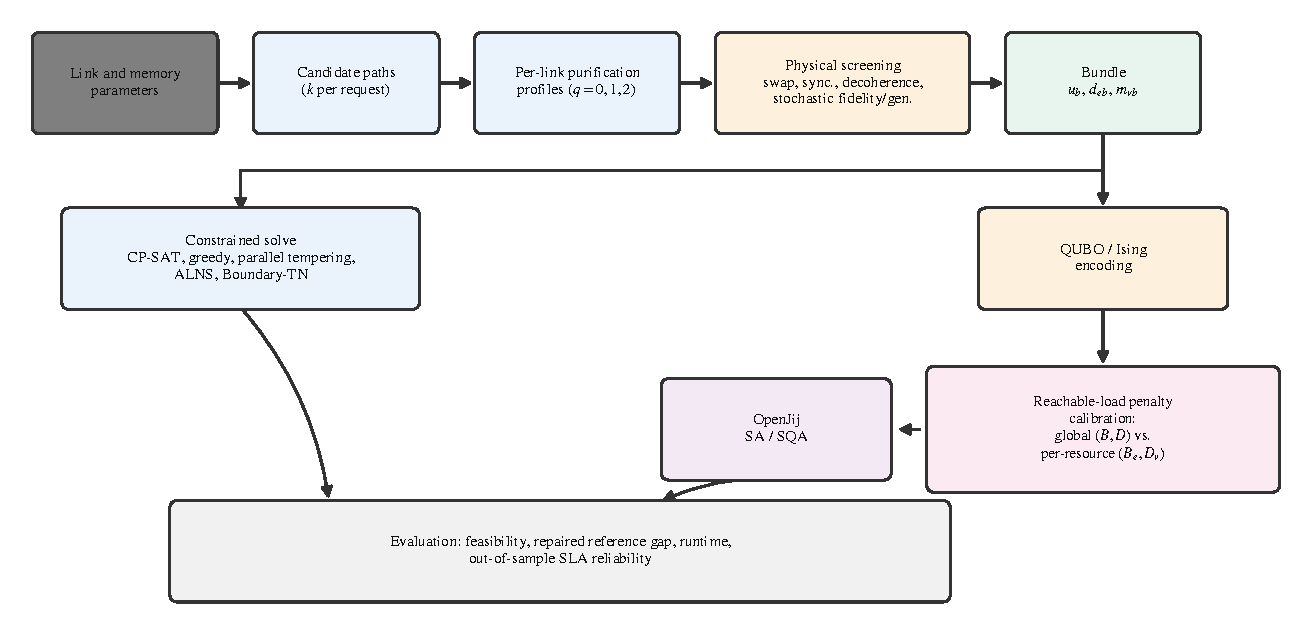
\includegraphics[width=0.98\textwidth]{fig1_workflow.pdf}
\caption{\textbf{QiOpt4QNet workflow.} Physical link and memory parameters define candidate paths. Each path is expanded into per-link purification profiles, screened under swapping, synchronization, memory decoherence and stochastic fidelity/generation scenarios, and converted into a bundle with utility and resource demands. Allocation is solved either directly as a constrained problem or through a QUBO/Ising representation. The proposed calibration assigns resource-specific edge and memory penalties using reachable co-loads. Final evaluations report feasibility, reference gap, runtime and out-of-sample SLA reliability.}
\label{fig:workflow}
\end{figure*}


\section{Related work and positioning}\label{sec:related}

\subsection{Entanglement routing, purification and network utility}

Quantum-network routing differs from classical packet routing because a path is valuable only insofar as the network can create, store and transform a quantum resource of sufficient quality. Early repeater architectures established the loss--memory--operation trade-offs that make this distinction unavoidable\cite{briegel1998,dur1999,sangouard2011,azuma2023}. At the network layer, Pant \emph{et al.} showed that entanglement generation can benefit from network-level multipath structure rather than a single fixed chain\cite{pant2019}. Li \emph{et al.} subsequently combined multiple candidate paths, finite edge capacities and purification, comparing resource-allocation strategies for simultaneous requests\cite{li2021}. High-fidelity and optimal-routing formulations have continued this line by making fidelity guarantees and resource allocation explicit\cite{halder2024}, and the recent path-based entanglement-purification model of Halder \emph{et al.} treats purification decisions as part of online end-to-end resource allocation\cite{halder2026}.

Purification is especially important because fidelity improvement consumes multiple elementary pairs and therefore couples a local physical operation to network-wide capacity. Xiao \emph{et al.} introduced Purification Scheduling Control, coordinating purification across concurrent requests to improve throughput under contention\cite{xiao2024}. Our bundle representation is complementary: it precomputes path-specific, per-edge purification profiles and exposes their edge/memory demands to the allocation optimizer. The present paper does not claim to reproduce PSC; rather, it uses the same systems insight that purification must be evaluated jointly with shared-resource constraints.

A separate but closely related literature formulates quantum resource allocation through network utility. Vardoyan and Wehner introduced quantum network utility maximization (QNUM), in which entanglement rate and quality jointly determine user utility\cite{vardoyan2023}. Kar and Wehner identified convexifiable cases of QNUM\cite{kar2025}, and Kar and Mukhopadhyay recently extended utility optimization to route selection itself through a mixed-integer convex formulation and randomized rounding\cite{kar2026}. Lo Piparo \emph{et al.} further emphasize quality-of-service behavior in aggregated quantum networks\cite{lopiparo2025}. QiOpt4QNet sits in this resource-allocation lineage but makes a different modeling choice: it discretizes each request into physically screened path--purification bundles, which makes heterogeneous purification and memory demand explicit and permits a common candidate set to be passed to exact, heuristic, tensor-network and QUBO solvers.

Recent surveys document a broad spectrum of reactive, proactive, opportunistic and virtual-routing strategies, as well as the growing importance of swapping probability, purification, memory lifetime and heterogeneous hardware\cite{abane2025}. These works motivate our use of a deliberately modular physical screen. We do not attempt to replace full-stack simulators. NetSquid\cite{coopmans2021} and SeQUeNCe\cite{wu2021} support detailed discrete-event modeling of hardware and protocols; our analytic evaluator instead provides a reproducible controlled layer for optimization studies, with the explicit future requirement of simulator-level cross-validation. Stochastic automatic-differentiation approaches to quantum-repeater design also illustrate the value of differentiable or optimizable physical surrogates when full simulations are random and expensive\cite{avis2025}.

\subsection{QUBO penalties and constrained annealing}

QUBO and Ising formulations translate constrained binary optimization into energy minimization and provide a common representation for simulated annealing, quantum annealing and specialized digital/analog optimizers\cite{lucas2014,glover2019,kirkpatrick1983,kadowaki1998}. The translation is not innocuous. Hard constraints are typically encoded by nonnegative penalty functions, so the chosen coefficient must be large enough to make every infeasible ground state unattractive. A coefficient that is unnecessarily large, however, reduces the relative dynamic range of the original objective and can degrade finite-precision or heuristic sampling.

Penalty selection has therefore become an optimization topic in its own right. Verma and Lewis study penalty magnitude and partitioning to improve QUBO solver performance\cite{verma2022}; Diez Garc{\'i}a \emph{et al.} derive exact and sequential penalty weights for constrained QUBOs\cite{diez2022}. Alessandroni \emph{et al.} formalize the ``quantum Big-M'' problem and show why exaggerated constraint scales are particularly undesirable when an encoded Hamiltonian must fit a physical or algorithmic energy range\cite{alessandroni2025}. Our contribution is narrower but structural: because QiOpt4QNet has a multiple-choice request structure and local edge/memory capacities, the set of co-loads that can actually occur on a given resource is sparse. We exploit that reachable-load structure to derive one sufficient coefficient per resource. The global-resource-aware arm in our experiment is a necessary control because it uses the same local derivation but collapses the values back to one family-wide maximum; it tightens a coefficient in only a minority of instances and changes solver behavior far less than the per-resource rule, which shows empirically that coefficient \emph{scope} matters in addition to coefficient \emph{derivation}.

\subsection{Tensor networks and hybrid combinatorial search}

Tensor networks offer a classical representation of high-dimensional states whose practical cost is controlled by entanglement/bond structure\cite{white1992,vidal2003,schollwock2011,orus2014}. Their use in combinatorial optimization is expanding. Hao \emph{et al.} map locally constrained optimization to a quantum-inspired tensor-network construction\cite{hao2022}; Nakada \emph{et al.} design tensor networks whose support is restricted to feasible configurations\cite{nakada2025}; and Preisser \emph{et al.} recently combine variational product/MPS ans{"a}tze with iterated local search on large combinatorial problems\cite{preisser2026}. Rosales applies Hamiltonian, Monte Carlo and stochastic boundary-MPS ideas to QKD routing\cite{rosales2026}. These studies motivate tensor-network search as a structured approximation, but none makes a general promise that MPS compression will outperform problem-specific classical solvers.

Our experiments are designed around that caution. Boundary-TN is evaluated before hybrid refinement and across a controlled width sweep; a separate SVD/MPS implementation is run with greedy fallback disabled. HybridBoundaryTN+ALNS is reported as a different algorithm, not as tensor-network performance. This distinction matters because a good compressed initializer and a good exact-neighborhood repair can be jointly useful even when the raw compressed solution is not competitive.

\subsection{Robust and chance-constrained network control}

Chance-constrained programming dates to Charnes and Cooper\cite{charnes1959}, while robust optimization formalizes the trade-off between nominal objective value and protection against uncertain data\cite{bertsimas2004}. Quantum networks provide a natural application: an allocation is useful only if its realized entanglement quality satisfies application requirements, yet fidelity, generation time and operation success are uncertain. Existing routing work increasingly treats fidelity as a first-class constraint\cite{li2021,halder2024,halder2026}, but most algorithmic benchmarks still report deterministic or in-sample quantities. Our reliability experiment therefore uses two scenario layers: scenarios used during candidate scoring/screening and an independent Monte Carlo stream used only for evaluation. The resulting SLA-violation rate is not a device-independent probability guarantee; it is an out-of-sample reliability metric under a declared stochastic physical model.

\section{Results}\label{sec:results}

\subsection{A physics-aware bundle model separates network control from physical screening}

Each request $r\in\Rset$ specifies a source, destination, priority $w_r$ and minimum end-to-end fidelity $F_r^{\min}$. Rather than optimizing path edges and purification rounds in one monolithic nonlinear model, QiOpt4QNet enumerates a finite bundle set $\Bset_r$. A bundle $b\in\Bset_r$ contains a candidate path $p_b$, one purification depth $q_{e,b}\in\{0,1,2\}$ for each path edge, predicted end-to-end fidelity and success probability, latency, an edge-demand vector $d_{e b}$, a node-memory demand vector $m_{v b}$, and a nominal or robust utility $u_b$. The allocation decision $x_b\in\{0,1\}$ then obeys
\begin{align}
\max_x\quad &\sum_b u_bx_b,\label{eq:allocobj}\\
\text{s.t.}\quad &\sum_{b\in\Bset_r}x_b\le 1 &&\forall r\in\Rset,\label{eq:req}\\
&\sum_b d_{eb}x_b\le C_e &&\forall e\in\Eset,\label{eq:edgecap}\\
&\sum_b m_{vb}x_b\le M_v &&\forall v\in\Vset.\label{eq:memcap}
\end{align}
This decomposition is useful because the physics evaluator can be upgraded independently of the optimizer, while all solver families see exactly the same candidate table and hard capacities.

The screening model is deliberately transparent rather than a claim of hardware-complete simulation. Elementary generation probability decreases with fiber attenuation and includes source, coupling and detection efficiencies. Purification follows the standard BBPSSW recurrence\cite{bennett1996}; if a link with Werner-like fidelity $F$ undergoes one round, the success proxy is
\begin{equation}
 p_{\mathrm{pur}}(F)=F^2+\frac{2F(1-F)}{3}+5\left(\frac{1-F}{3}\right)^2,
\end{equation}
and the conditional output fidelity is
\begin{equation}
 F'=\frac{F^2+[(1-F)/3]^2}{p_{\mathrm{pur}}(F)}.
\end{equation}
A depth $q$ consumes $2^q$ raw pairs. Prepared links are synchronized before swapping; early links therefore wait in memory. For an initial Werner-like Bell fidelity $F_0$, the shared storage model is
\begin{equation}
F(t)=\frac14+\left(F_0-\frac14\right)\eta(t),\qquad
\eta(t)=e^{-t/T_2}\frac{1+e^{-t/T_1}}{2},\label{eq:memory}
\end{equation}
with $T_1=2T_2$ in the default benchmark. Equation~\ref{eq:memory} satisfies $F(0)=F_0$ and approaches the maximally mixed Bell overlap $1/4$ at long storage times. Two links are swapped using the Werner composition
\begin{equation}
F_{12}^{\mathrm{ideal}}=F_1F_2+\frac{(1-F_1)(1-F_2)}{3},
\end{equation}
followed by a local depolarizing operation of quality $\eta_s$,
$F_{12}=\eta_sF_{12}^{\mathrm{ideal}}+(1-\eta_s)/4$.
Path success multiplies purified-link success proxies and one swap-success factor for each intermediate swap.

We subjected these equations to an internal independent-formulation audit before using them in optimization. The frozen physics validation used 150,000 Monte Carlo samples, passed all memory invariants, and yielded maximum absolute errors of $4.44\times10^{-16}$ for the density-matrix fidelity cross-check and $1.11\times10^{-16}$ for the swap cross-check. These tests validate implementation consistency, not calibration to a specific experimental platform. Full protocol simulators such as NetSquid\cite{coopmans2021} and SeQUeNCe\cite{wu2021} model hardware/control stacks at finer granularity; external simulator cross-validation is therefore a limitation and an important next step.

\begin{table}[t]
\caption{Default physical screening parameters used for journal instances. The model is technology-agnostic and intended for controlled algorithmic comparison rather than device-specific prediction.}\label{tab:physics}
\centering
\small
\begin{tabular}{@{}ll@{}}
\toprule
Parameter & Default value\\
\midrule
Fiber attenuation & $0.20$ dB km$^{-1}$\\
Source / coupling / detector efficiency & $0.98 / 0.97 / 0.95$\\
Swap success probability & $0.96$\\
Swap operation fidelity & $0.992$\\
Swap operation time & $5\,\mu$s\\
Memory coherence $T_2$ & $6000\,\mu$s\\
Memory relaxation $T_1$ & $2T_2$\\
Attempt rate & $2\times10^5$ s$^{-1}$\\
Epoch duration & $25$ ms\\
Fidelity perturbation s.d. & $0.008$\\
Generation lognormal s.d. & $0.10$\\
Maximum purification depth & $2$ rounds/link\\
SLA probability threshold & $0.80$\\
\bottomrule
\end{tabular}
\end{table}

\subsection{Strong classical optimizers define the practical reference regime}

We first compared solvers on six benchmark regimes spanning 14--100 nodes and 12--80 requests. Exact bottleneck and geometric instances contain 14--16 nodes and 12--14 requests; medium instances contain 32--40 nodes and 32--36 requests; large instances contain 80--100 nodes and 72--80 requests. Exact and medium regimes used ten independently generated seeds each, and large regimes five. Exact CP-SAT certificates were used where practical; otherwise the best observed feasible utility among the compared solvers was used as a reference and was labelled accordingly.

The result is not a quantum-inspired dominance story. CP-SAT, AdaptiveLNS, HybridBoundaryTN+ALNS and parallel tempering reached zero mean gap across the four exact/medium aggregate cells; in the larger geometric regime, parallel tempering differed from the best-observed reference by only $0.0003\%$ (Fig.~\ref{fig:benchmark}; Table~\ref{tab:benchmark}). Greedy-fidelity was also unexpectedly strong on these benchmark aggregates: its gap was 0\% in exact-bottleneck, $0.012\%$ in exact-geometric, $0.53\%$ in medium-bottleneck and $0.15\%$ in medium-Waxman. Thus, on many tested instances, the physical candidate construction already exposes enough structure that a strong feasible heuristic captures most of the available utility.

The stochastic boundary tensor-network (Boundary-TN) method was competitive in some structured cases but less uniform: mean gaps were $5.89\%$ for exact-bottleneck, $0\%$ for exact-geometric, approximately $4$--$1\%$ across medium cells, $11.87\%$ on large-bottleneck and $0.60\%$ on large-geometric. By contrast, the calibrated OpenJij SQA ensemble remained far from the classical reference: $38.80\%$, $49.99\%$, $48.93\%$ and $47.03\%$ mean gaps on exact-bottleneck, exact-geometric, medium-bottleneck and medium-Waxman, respectively. Its median wall times were orders of magnitude larger than the strongest classical methods in these cells. These results are a useful negative control: a QUBO/annealing representation does not itself confer competitive performance.

\begin{figure*}[t]
\centering
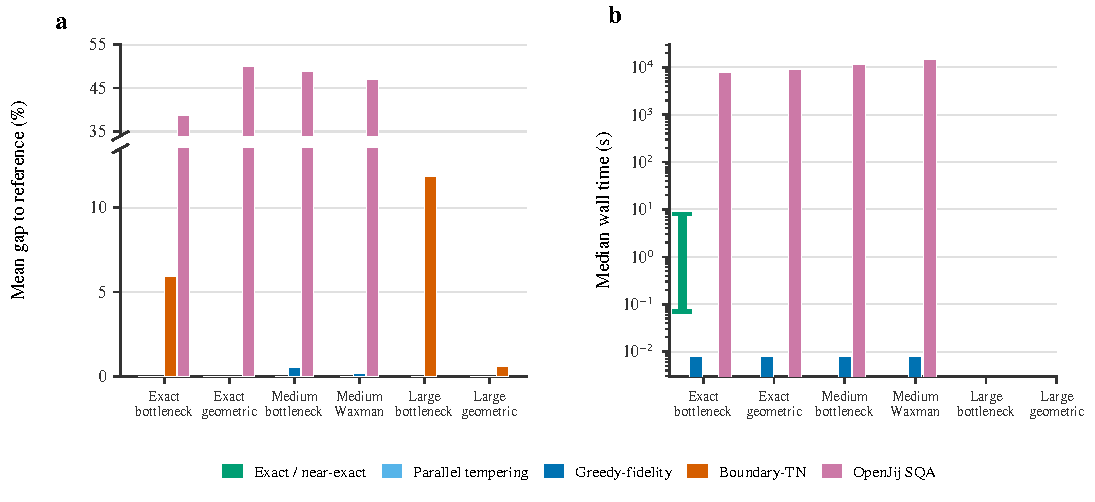
\includegraphics[width=0.96\textwidth]{fig4_solver_benchmark.pdf}
\caption{\textbf{Solver quality and runtime across accepted benchmark regimes.} Left: mean gap to the certified CP-SAT optimum in exact regimes or the stated best-observed reference in larger regimes. Right: median wall time on a logarithmic scale. Strong constrained optimizers and parallel tempering reach or closely track the reference, while the OpenJij SQA ensemble remains substantially behind on the exact/medium cells in which it was run. Missing solver/regime combinations were not executed and are not imputed.}
\label{fig:benchmark}
\end{figure*}

\begin{table*}[t]
\caption{Selected accepted benchmark results. Gaps are relative to CP-SAT optimal utility where certified and otherwise to the best observed feasible solution. Values are aggregate means over the listed regime seeds.}\label{tab:benchmark}
\centering
\small
\resizebox{\textwidth}{!}{%
\begin{tabular}{@{}llllrr@{}}
\toprule
Regime & Size & Solver & Mean utility & Mean gap (\%) & Median wall time (s)\\
\midrule
Exact bottleneck & 14 nodes, 12 req. & CP-SAT / LNS / Hybrid / PT & 64.27 & 0.00 & $\sim0.07$--8\\
& & Greedy-fidelity & 64.27 & 0.00 & $<0.01$\\
& & Boundary-TN & 62.09 & 5.89 & ---\\
& & OpenJij SQA ensemble & 38.81 & 38.80 & 7877\\
\addlinespace
Exact geometric & 16 nodes, 14 req. & CP-SAT / LNS / Hybrid / PT & 299.62 & 0.00 & ---\\
& & Greedy-fidelity & 299.58 & 0.012 & $<0.01$\\
& & Boundary-TN & 299.62 & 0.00 & ---\\
& & OpenJij SQA ensemble & 146.66 & 49.99 & 9191\\
\addlinespace
Medium bottleneck & 32 nodes, 32 req. & CP-SAT / LNS / Hybrid / PT & 163.70 & 0.00 & ---\\
& & Greedy-fidelity & 162.86 & 0.53 & $<0.01$\\
& & OpenJij SQA ensemble & 85.04 & 48.93 & 11544\\
\addlinespace
Medium Waxman & 40 nodes, 36 req. & CP-SAT / LNS / Hybrid / PT & 437.54 & 0.00 & ---\\
& & Greedy-fidelity & 437.06 & 0.15 & $<0.01$\\
& & OpenJij SQA ensemble & 231.30 & 47.03 & 14978\\
\addlinespace
Large bottleneck & 80 nodes, 72 req. & LNS / Hybrid / PT & 194.97 & 0.00 & ---\\
& & Boundary-TN & 171.78 & 11.87 & ---\\
Large geometric & 100 nodes, 80 req. & LNS / Hybrid & 1193.05 & 0.00 & ---\\
& & Parallel tempering & 1193.05 & 0.0003 & ---\\
& & Boundary-TN & 1185.92 & 0.60 & ---\\
\bottomrule
\end{tabular}%
}
\end{table*}

A separate hardness sweep covered 768 solver-instance rows across request counts $12$--$52$, four capacity scales and eight seeds per cell. Over this sweep, mean gaps were $1.07\%$ for Greedy-scarcity, $5.89\%$ for Boundary-TN, $0.035\%$ for AdaptiveLNS and $0.022\%$ for the Boundary-TN+ALNS hybrid. Median runtimes were approximately $0.0014$, $4.88$, $4.20$ and $7.46$ s, respectively. Greedy degradation increased under tighter capacities in some cells, but the observed transition was moderate rather than catastrophic: the largest mean greedy cell gap was about $2.94\%$. The defensible conclusion is therefore that strong greedies are sufficient for many instances, whereas exact-neighborhood/global search reduces the tail of allocation errors under tighter coupling.

\subsection{Tensor-network compression exhibits a quality--runtime frontier, not universal superiority}

To isolate tensor-network behavior from hybrid post-processing, we varied the retained Boundary-TN width $\chi$ with no fallback. Mean gap to the LNS reference decreased overall from $13.19\%$ at $\chi=8$ to $5.00\%$ at $\chi=256$, while median runtime increased from $0.33$ s to $11.27$ s (Fig.~\ref{fig:tn}). Intermediate widths $(16,32,64,128)$ yielded mean gaps of $13.13\%$, $9.11\%$, $8.13\%$ and $7.79\%$. This supports a practical compression frontier: retaining more boundary states captures more interaction structure but consumes more time and memory.

We also ran an explicit SVD/MPS ablation to guard against a common benchmarking ambiguity in which a purported tensor-network solver silently returns a greedy repair. The experiment spans $\chi\in\{2,4,8,16,32,64\}$ and one, two or four SVD sweeps (180 rows total); greedy fallback was disabled and was never used. MPS quality was not monotonic in $\chi$ or sweep count, and in representative cells the repaired MPS remained below the greedy baseline (for example, seed 0, $\chi=8$, one sweep: raw MPS utility 67.40 versus greedy 70.51). This negative result is scientifically informative: tensor-network representations can be useful as compression/initialization mechanisms, but their effectiveness depends on the induced interaction ordering and retained bond dimension. Recent MPS optimization studies similarly emphasize that ansatz structure and the surrounding search strategy determine performance\cite{preisser2026}.

\begin{figure*}[t]
\centering
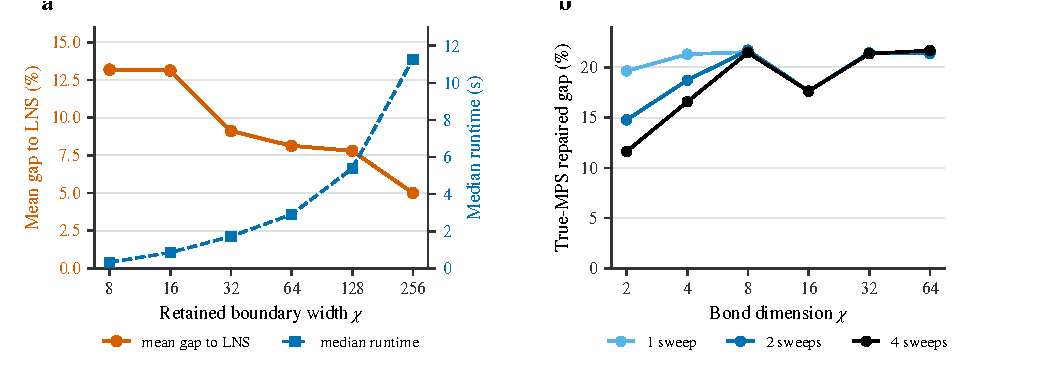
\includegraphics[width=0.96\textwidth]{fig6_tn_diagnostics.pdf}
\caption{\textbf{Tensor-network diagnostics.} Left: Boundary-TN mean reference gap decreases as retained width $\chi$ grows, while runtime increases, giving an explicit compression frontier. Right: true SVD/MPS ablations across sweep counts show non-monotonic quality and no hidden greedy fallback. The tensor-network contribution is therefore interpreted as structured approximation and initialization rather than unconditional solver superiority.}
\label{fig:tn}
\end{figure*}

\subsection{Reliability-aware selection trades nominal utility for fewer out-of-sample SLA failures}

A bundle selected because its nominal predicted fidelity exceeds $F_r^{\min}$ may still violate the request threshold when raw link fidelity or generation conditions drift. We compared three allocation policies on the same candidate physics: (i) \emph{nominal}, which optimizes the deterministic bundle utility; (ii) \emph{robust}, which weights expected scenario utility by the in-sample SLA probability and subtracts a fidelity-shortfall penalty; and (iii) \emph{chance}, which additionally screens candidate bundles by an empirical fidelity-SLA probability threshold. Crucially, selected plans were evaluated on an independent Monte Carlo stream rather than the scenarios used to construct them.

Across 36 accepted runs, nominal allocation achieved the highest mean optimization utility (124.25) but also the highest out-of-sample SLA violation rate (16.3\%). The robust policy reduced violations to 12.1\% at mean utility 114.51. The chance-constrained policy reduced violations further to 6.0\%, with mean utility 115.64 and slightly higher delivered fidelity (0.863 versus 0.860 nominal). Relative to nominal, chance-constrained selection therefore cut the observed violation rate by about 63\% while sacrificing 6.9\% of optimization utility (Fig.~\ref{fig:robust}). This is an empirical ``price of robustness'' in the quantum-network setting\cite{bertsimas2004}: reliability is valuable but not free.

The result also clarifies the role of chance constraints. The constraint is not a claim that empirical sampling exactly proves a hardware-level reliability guarantee; it is a controlled screen under the stated stochastic model. Nevertheless, separating optimization scenarios from the validation stream prevents the strongest form of in-sample optimism and exposes the trade-off a controller would face when setting a service-level risk tolerance.

\begin{figure*}[t]
\centering
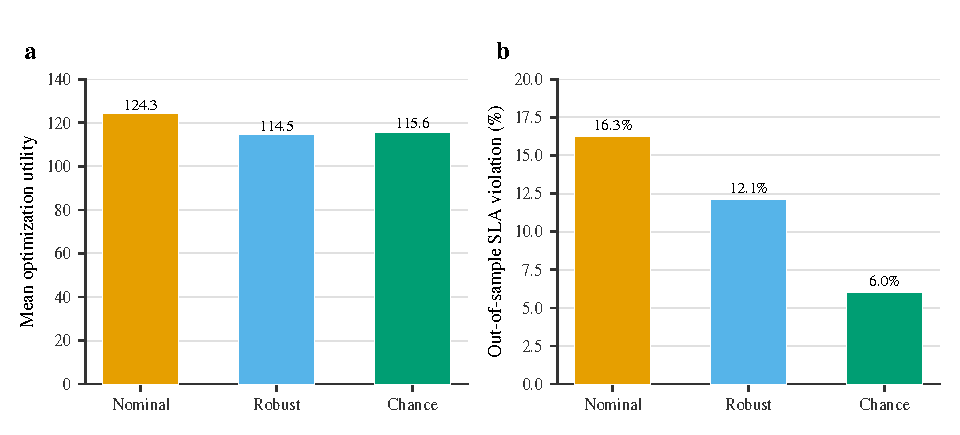
\includegraphics[width=0.88\textwidth]{fig5_robustness.pdf}
\caption{\textbf{Nominal utility versus out-of-sample reliability.} Mean optimization utility (left) and independently sampled fidelity-SLA violation rate (right) for nominal, robust-objective and chance-constrained policies. Chance-constrained selection lowers observed violations from 16.3\% to 6.0\% while retaining 93.1\% of nominal optimization utility.}
\label{fig:robust}
\end{figure*}

\subsection{Resource-specific QUBO calibration avoids the global Big-M bottleneck}

For annealing-based optimization, Eqs.~\ref{eq:req}--\ref{eq:memcap} are embedded into an unconstrained energy. Let $P_0=\max_b u_b^+$ be the largest positive bundle utility. A transparent conventional rule uses $A=B=D=P_0+\eps$ for the at-most-one, edge-capacity and memory-capacity penalties. This guarantees that a single profitable bundle cannot compensate for the smallest unit hard-constraint penalty, but it assigns every capacity constraint the scale required by the globally most valuable bundle.

We instead exploit the discrete load structure of each resource. Consider resource $j$ with capacity $C_j$ and a candidate bundle $b$ of demand $d_{jb}$. Because at most one bundle can be selected per request, define $\mathcal{L}_{j,-r(b)}$ as the set of co-loads reachable by selecting zero or one bundle from every request other than $r(b)$. For a co-load $\ell$, removing $b$ from a violated squared-overload penalty changes that penalty by
\begin{equation}
\Delta_{j,b}(\ell)= [\max(0,\ell+d_{jb}-C_j)]^2-[\max(0,\ell-C_j)]^2.\label{eq:delta}
\end{equation}
Among reachable co-loads for which $\ell+d_{jb}>C_j$, the smallest violating $\ell$ produces the weakest useful penalty drop for the implementation's squared-overload structure. We therefore define
\begin{equation}
B_j=\max_{b:\,d_{jb}>0}\frac{u_b^+}{\Delta_{j,b}}+\eps,\label{eq:resourceB}
\end{equation}
where $\Delta_{j,b}$ is evaluated at that smallest reachable violating co-load. Edge coefficients use $B_e$ and node-memory coefficients use $D_v$ analogously. Request-conflict coefficient $A$ remains $P_0+\eps$. A global resource-aware control takes the maximum of these bounds over all edges (and separately all memories), so that $B_{\mathrm{global}}=\max_e B_e$; the proposed \emph{per-resource} rule retains them individually.

\begin{proposition}[Ground-state sufficiency]\label{prop:ground}
Assume nonnegative integer resource demands and capacities, at most one bundle per request, zero soft-congestion weights ($C=E=0$), and coefficients in Eq.~\ref{eq:resourceB} with strictly positive margin $\eps$. Then any global minimum of the QUBO energy is feasible with respect to the corresponding edge and memory capacity constraints, and, with $A>P_0$, request conflicts are excluded as well. Consequently the ground state attains the constrained optimal utility.
\end{proposition}
\noindent\textit{Proof sketch.} Suppose a selected state violates resource $j$. Choose any selected bundle $b$ participating in that violation for which the request-conditioned co-load is reachable. Removing $b$ loses at most $u_b^+$ in objective value but reduces the resource penalty by $B_j\Delta_{j,b}>u_b^+$. Loads on other resources cannot increase after removal. The resulting state has strictly lower energy, so an infeasible state cannot be a global minimum. A request containing two selected bundles can similarly lower energy by dropping one because the pairwise request-conflict penalty exceeds the largest positive utility. $\square$

\begin{remark}
The assumption $C=E=0$ is essential to the last statement of the proposition. Soft congestion terms penalize feasible loads, so with positive weights the ground state need not be utility-optimal, and no optimality guarantee is claimed. All calibration experiments reported here therefore set $C=E=0$.
\end{remark}

We did not rely on the proof sketch alone. Randomized tiny instances were exhaustively enumerated and compared against constrained optima; all 2,000 ground-state audit cases passed. This includes request conflicts as well as edge and memory overloads.

The complete calibration experiment generated 1,080 valid instances (four topology/capacity configurations, 90 generation seeds and request counts 8, 16 and 24). A scan of the coefficients found that at least one edge and one memory coefficient was strictly tighter under the per-resource rule in 1,078 of them; these 1,078 were solved under conventional, global resource-aware and per-resource calibration using both SA and SQA, five solver seeds and 100 requested reads, yielding 32,340 solver rows. Selection depended only on whether coefficients changed, not on solver performance. In the two remaining instances no coefficient is tighter under any rule, so they carry no information about the treatment. Solver seeds were treated as repeated measurements: they were averaged within each generated instance before statistical inference. Because a generation seed is reused across topology/load cells, confidence intervals resampled the 90 generation-seed blocks rather than individual rows.

Per-resource calibration materially reduced hard-constraint scales (Fig.~\ref{fig:coeff}). Averaged over all 1,080 instances, the per-resource rule lowered the mean edge and memory coefficients by 49.5\% and 46.3\% relative to the conventional coefficient, whereas the global control lowered them by only 4.3\% and 3.0\%. Across individual resources, 88.7\% of edge coefficients and 80.3\% of memory coefficients were tightened. This is an average over each instance's resources (on average 12.4 edges and 10.4 memories, of which 11.0 and 8.3 are tightened): it reflects lowering \emph{non-binding} penalties. It is not a reduction of the binding penalty, which is impossible under this construction because $B_{\mathrm{global}}=\max_eB_e$. Tightening was strongest at low load: mean per-resource edge/memory ratios to the conventional coefficient were $0.352/0.350$ at 8 requests, $0.531/0.575$ at 16 and $0.631/0.686$ at 24, while the global ratios were $0.889/0.914$, $0.986/0.996$ and $0.997/1.000$. The mechanism is intuitive: as more requests are available, reachable co-load sets become denser, making unit penalty drops more common and leaving less room below the conventional global scale.

\begin{figure*}[t]
\centering
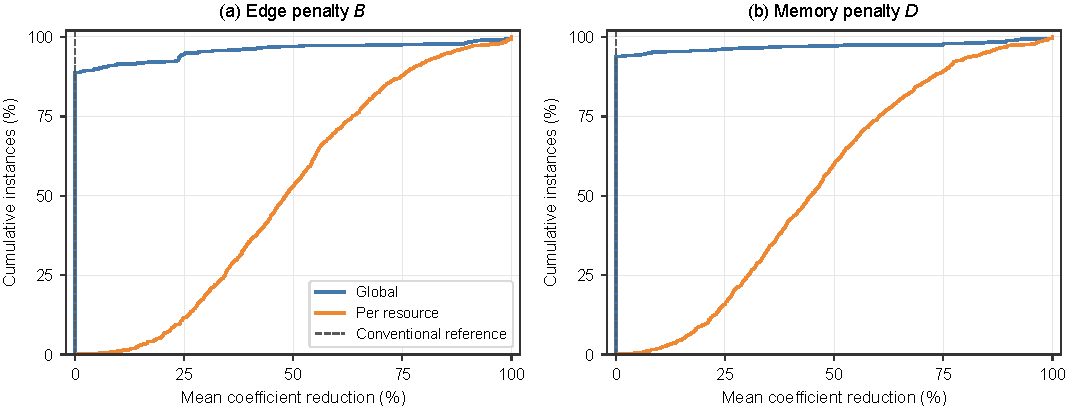
\includegraphics[width=0.60\textwidth]{figure2_coefficient_ratios.pdf}
\caption{\textbf{Resource-specific penalty tightening.} Empirical cumulative distributions of coefficient reductions across all 1,080 instances. Each edge observation is $100(1-\overline B/B_{\mathrm{ref}})$, with the analogous expression for memory; the observation is the within-instance mean over modeled resources, and for the global rule it equals the single family coefficient. Zero reductions are included. Keeping coefficients per edge and per memory exposes substantially smaller local sufficient penalties, especially at lower load, whereas the global maximum is pinned by a single difficult resource.}
\label{fig:coeff}
\end{figure*}

\subsection{Per-resource calibration improves annealing feasibility and repaired quality}

The coefficient reduction translated into a strong SA effect and a smaller SQA effect (Fig.~\ref{fig:calib-effects}; Table~\ref{tab:calib-main}). Relative to conventional calibration, per-resource calibration raised the SA raw feasible-read rate from 0.2397 to 0.3597 (paired difference $+0.1200$, generation-seed-block bootstrap 95\% CI $[0.1044,0.1354]$) and lowered the repaired reference gap from 86.30\% to 75.47\%, a difference of $-10.84$ percentage points (pp; CI $[-11.67,-9.98]$). For SQA, the feasible-read rate rose from 0.3874 to 0.4631 ($+0.0757$, CI $[0.0575,0.0940]$) and the repaired gap fell from 29.69\% to 22.94\% ($-6.75$ pp, CI $[-7.51,-6.01]$). Per-resource calibration was better in 71.7\% (SA) and 74.4\% (SQA) of instances by repaired gap, and worse in 24.0\% and 25.6\%.

\begin{table}[t]
\caption{Paired solver effects on the 1,078 evaluated instances (five solver seeds averaged per instance); 95\% generation-seed-block bootstrap intervals in brackets. Feasibility and gap are in percentage points; overload is in raw resource units. Lower is better for gap and overload. PR = per-resource, G = global, C = conventional.}\label{tab:calib-main}
\centering
\footnotesize
\begin{tabular}{@{}llccc@{}}
\toprule
Contrast & Sampler & Feasible rate (pp) & Repaired gap (pp) & Raw overload\\
\midrule
PR $-$ C & SA & $+12.00\ [10.44,13.54]$ & $-10.84\ [-11.67,-9.98]$ & $-1.5325\ [-1.6731,-1.3896]$\\
PR $-$ C & SQA & $+7.57\ [5.75,9.40]$ & $-6.75\ [-7.51,-6.01]$ & $+0.0178\ [-0.0000,0.0381]$\\
PR $-$ G & SA & $+11.60\ [10.05,13.15]$ & $-10.33\ [-11.20,-9.46]$ & $-1.5338\ [-1.6796,-1.3855]$\\
PR $-$ G & SQA & $+6.86\ [5.15,8.63]$ & $-5.95\ [-6.58,-5.35]$ & $+0.0173\ [0.0004,0.0362]$\\
G $-$ C & SA & $+0.41\ [0.07,0.78]$ & $-0.50\ [-0.82,-0.22]$ & $+0.0013\ [-0.0204,0.0256]$\\
G $-$ C & SQA & $+0.71\ [0.13,1.30]$ & $-0.80\ [-1.19,-0.45]$ & $+0.0006\ [-0.0028,0.0041]$\\
G $-$ C, 127 changed & SA & $+3.46\ [0.63,6.56]$ & $-4.27\ [-6.98,-1.94]$ & $+0.0110\ [-0.1687,0.2276]$\\
G $-$ C, 127 changed & SQA & $+5.98\ [1.33,10.79]$ & $-6.77\ [-9.96,-3.88]$ & $+0.0047\ [-0.0228,0.0344]$\\
\bottomrule
\end{tabular}
\end{table}

Because the global rule is itself a reachable-load rule, the conventional baseline conflates two things: adopting reachable-load calibration at all, and scoping it per resource. We therefore report the direct contrast. Per-resource calibration raised the raw feasible-read rate by 11.60 pp (SA, CI $[10.05,13.15]$) and 6.86 pp (SQA, CI $[5.15,8.63]$) over the global rule and lowered the repaired gap by 10.33 pp ($[-11.20,-9.46]$) and 5.95 pp ($[-6.58,-5.35]$). Nearly all of the effect measured against the conventional reference is therefore attributable to keeping the coefficient per resource, rather than to the reachable-load bound as such.

The global rule's pooled effect against conventional calibration is small ($+0.41$ and $+0.71$ pp in feasibility, $-0.50$ and $-0.80$ pp in gap) but this is a dilution: 951 of the 1,078 evaluated instances (88.2\%) have coefficients identical to the conventional reference under the global rule, because they were selected on the per-resource criterion, and contribute exact zeros. Restricted to the 127 instances where the global rule changed a coefficient, it raises feasibility by 3.46 pp (SA) and 5.98 pp (SQA) and lowers the repaired gap by 4.27 and 6.77 pp (Table~\ref{tab:calib-main}, last two rows). The global rule therefore helps where it acts; it simply acts rarely, and where it acts the per-resource gain against it is still larger.

Per-resource calibration also lowered mean SA raw overload by 1.53 resource units, but it did \emph{not} lower SQA raw overload: against the global rule it raised it slightly (mean $+0.017$ units, 95\% CI $[0.0004,0.0362]$), and against the conventional rule the change was indistinguishable from zero (CI lower bound $-5\times10^{-19}$). Importantly, even calibrated SQA did \emph{not} close the gap to CP-SAT/LNS/PT in the separate journal benchmark, and mean repaired reference gaps under per-resource calibration remain 75.5\% (SA) and 22.9\% (SQA) on this study. Penalty calibration should therefore be interpreted as an encoding improvement, not as evidence that annealing is the best solver for this application.

Two features of the solver protocol affect how these numbers should be read. First, with a fixed seed, OpenJij's SA and SQA return \emph{identical} reads within a call: requesting 1, 100 or 1,000 reads returns that many samples, but all are the same state (one distinct sample). A ``100-read'' call is therefore one sample per solver seed, every archived call is uniformly feasible or uniformly infeasible, and the read budget is not a budget in the usual sense (Methods). Second, we report 24 paired comparisons (3 contrasts $\times$ 2 samplers $\times$ 3 metrics, plus 6 for the restricted global contrast) with no multiplicity correction, so about one interval in twenty would be expected to exclude zero by chance; intervals reflect variation over generated instances only, with five fixed solver seeds averaged within each instance.

\begin{figure*}[t]
\centering
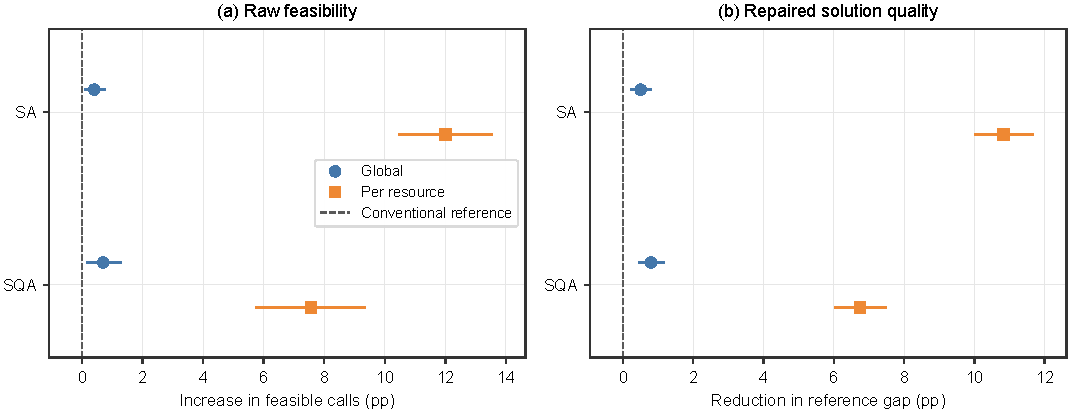
\includegraphics[width=0.60\textwidth]{figure3_solver_paired_effects.pdf}
\caption{\textbf{Paired effects of the calibration rules.} Paired solver effects on the 1,078 evaluated instances for three contrasts: global versus conventional, per-resource versus conventional, and per-resource versus global. Points show mean effects after averaging five matched seeded calls per instance; lines show pointwise 95\% generation-seed-block bootstrap intervals. Left: increase in raw feasibility. Right: reduction in repaired CP-SAT reference gap. Both axes use percentage points; positive values favor the first calibration named in each contrast.}
\label{fig:calib-effects}
\end{figure*}

\section{Discussion}\label{sec:discussion}

The experiments support a restrained but useful picture of quantum-network orchestration. First, the dominant practical distinction in the tested problem family is not ``quantum-inspired versus classical.'' Strong feasible greedy allocation is already close to optimal in many exact and medium regimes, and CP-SAT, ALNS, the TN-initialized ALNS hybrid and parallel tempering close nearly all remaining reference gaps. This indicates that expensive global optimization pays primarily as insurance against coupled resource conflicts and difficult tails, rather than as a universal requirement. The 768-row hardness sweep reinforces this interpretation: greedy quality worsens under tighter capacities, but the transition is moderate and instance-dependent.

Second, tensor networks are best viewed here as structured compression mechanisms. The Boundary-TN ablation shows a clear average quality/runtime trade-off as $\chi$ increases, while the true-MPS experiment shows that simply increasing a bond dimension or SVD sweep count does not guarantee monotonic improvement. This is consistent with the broader tensor-network optimization literature, in which encoding, variable ordering, feasibility structure and local-search integration are as important as the nominal tensor-network family\cite{hao2022,nakada2025,preisser2026}. A promising systems strategy is therefore hybrid: use compressed global structure to generate a good basin, then exploit exact or problem-specific local repair. Our Boundary-TN+ALNS results are consistent with that strategy, although the present benchmarks do not establish a universal runtime advantage.

Third, reliability should be treated as an explicit control objective. Quantum-network routing literature increasingly incorporates fidelity and purification\cite{li2021,xiao2024,halder2024,halder2026}, and network-utility formulations provide a natural language for assigning value to entanglement quality and rate\cite{vardoyan2023,kar2025,kar2026}. Our out-of-sample experiment adds a complementary observation: optimizing nominal service value alone can materially understate fidelity-SLA risk. Chance-constrained screening more than halves the observed violation rate in the tested stochastic model, but it sacrifices nominal utility. The correct operating point is therefore policy-dependent; the framework exposes the trade-off rather than prescribing one risk tolerance.

Fourth, penalty calibration is a meaningful optimization problem in its own right. Generic QUBO rules often use a single objective-scale penalty because it is simple and safe\cite{glover2019,verma2022}. Recent work on the quantum Big-M problem demonstrates why unnecessarily large coefficients can be harmful to quantum or quantum-inspired optimizers\cite{alessandroni2025}. Our result adds a resource-allocation-specific mechanism: when at-most-one-request structure restricts which co-loads are reachable, the smallest actual overload correction can be larger than the algebraic unit assumed by a global bound. A request-conditioned dynamic program exposes these gaps. Keeping the resulting coefficient local to each edge or memory is essential; otherwise an unrelated worst-case resource restores the global scale. This explains both the roughly twofold reduction in mean coefficients and why the global rule, which tightens a coefficient in only 127 of the 1,078 evaluated instances, produces a small pooled effect while the per-resource rule does not.

Several limitations delimit the conclusions. The physical model is an analytic screening model built around Werner-state fidelities, BBPSSW purification, independent stochastic link perturbations and a phenomenological $T_1/T_2$ memory envelope. It omits technology-specific effects such as multiplexing control overheads, correlated noise, finite classical-control queues, detailed detector dark counts and protocol-specific memory scheduling. The internal physics cross-checks are strong implementation tests but are not an external NetSquid/SeQUeNCe validation. The benchmark topologies are synthetic and the accepted core evidence does not support a claim of universal topology generalization: a separate topology-robustness artifact was incomplete at freeze time and is deliberately excluded. A planned Rosales-style extension was also incomplete and is not used for numerical comparison. Finally, OpenJij SQA is a classical simulator; the study contains no physical quantum-annealing experiment and no quantum speedup claim.

The calibration study has its own limits. The ground-state guarantee holds for $C=E=0$ and every experiment uses that setting; with positive soft-congestion weights the ground state need not be utility-optimal. The calibration study uses four small chain and grid configurations (8--16 nodes, 8--24 requests), so its topology generality is untested. Fixed-seed reads are identical, so solver variability is captured only by the five solver seeds and the read count does not act as a sampling budget; extra reads change nothing under this protocol. A separate check with independent reads (SA, all 1,078 instances, two solver seeds) found that the per-resource advantage does not shrink with more budget: $-13.2$ pp in repaired gap at 10 reads, $-13.1$ pp at 100 reads and $-15.8$ pp with ten times the sweeps (Supplementary Information); SQA was not included. The solver comparisons combine local utility bounds, redundant-constraint detection and reachable-load calculations, and their individual effects on annealing performance were not isolated. Per-resource calibration worsened instance-averaged repaired gaps in about 24--26\% of instances against conventional calibration and slightly increased raw SQA overload. Comparisons with other penalty-setting methods (for example the exact and sequential weights of Ref.~\cite{diez2022}) and broader solver-seed sets remain future work.

These limitations suggest concrete next steps rather than additional post hoc experiments for the present manuscript. The most valuable validation would be to replay a representative subset of selected bundles in a full-stack simulator and, eventually, on a hardware-informed testbed. Correlated memory/link noise could replace the independent scenario model, and larger networks could be studied with explicit distributed-control costs. On the optimization side, the per-resource calibration construction is not specific to quantum networking: it applies to multiple-choice, capacity-constrained QUBOs whenever request-conditioned reachable loads can be computed efficiently. Generalizing that theorem and testing it on multidimensional knapsack and other allocation problems is a separate methodological direction.

Overall, QiOpt4QNet argues for a systems view of quantum-network optimization. Fidelity, purification, memory and reliability determine which actions are physically credible; classical constrained optimization establishes a demanding reference; tensor-network and annealing methods should be evaluated against that reference without presuming advantage; and QUBO encodings themselves deserve structure-aware design. The resulting regime map is more useful than a single solver ranking: simple allocation is often enough, global/hybrid methods repair difficult coupling, chance constraints purchase reliability, and resource-specific QUBO penalties improve annealing behavior without changing the constrained problem being represented.

\section{Methods}\label{sec:methods}

\subsection{Network, requests and candidate paths}

A network is an undirected graph $G=(\Vset,\Eset)$. Each link stores distance, raw fidelity, elementary generation probability and an epoch Bell-pair capacity; each node stores a memory capacity. For every request, up to $k$ candidate simple paths are generated and expanded into purification profiles with at most two BBPSSW rounds per link. Profiles that are dominated, physically invalid or fail configured fidelity/SLA screening are removed. The journal regimes use $k=5$--6 and cap the retained bundle set at 16--18 bundles per request to control combinatorial growth. All random instances and their physical parameters are seeded and exported.

Elementary link generation uses
\begin{equation}
p_{\mathrm{gen}}(L)=\mathrm{clip}\!\left(\eta_s\eta_c\eta_d10^{-\alpha L/10}\,\xi,\,0.03,\,0.995\right),
\end{equation}
where $\alpha=0.20$ dB km$^{-1}$, $(\eta_s,\eta_c,\eta_d)=(0.98,0.97,0.95)$, and $\xi$ is a local link factor. The expected ready time for $n$ raw pairs with $m$ parallel modes is $n/(p_{\mathrm{gen}}mf_{\mathrm{attempt}})$, with $f_{\mathrm{attempt}}=2\times10^5$ Hz. Synchronization time is the maximum ready time over path links; links finishing earlier decohere according to Eq.~\ref{eq:memory}. Classical propagation contributes $4.9\,\mu$s per kilometer, and each swap adds $5\,\mu$s.

For a nominally evaluated bundle, the service term is
\begin{equation}
v_b=w_r p_b\left[1+\max(F_b-F_r^{\min},0)\right],
\end{equation}
and the utility is
\begin{equation}
u_b=v_b-\lambda_L L_b-\lambda_B N_b,
\end{equation}
with latency penalty $\lambda_L=0.0015$ and raw-Bell-pair penalty $\lambda_B=0.025$. The utility is a benchmark control objective, not an economic valuation of entanglement. It rewards success probability and fidelity margin while accounting for latency and pair consumption.

\subsection{Stochastic robustification and chance screening}

For robust candidate construction, raw fidelities receive independent Gaussian perturbations with standard deviation 0.008. Generation probabilities are multiplied by lognormal factors centered near one with log standard deviation 0.10. For scenarios $s=1,\ldots,S$, the evaluator returns $F_b^{(s)}$, $p_b^{(s)}$ and nominal utility $u_b^{(s)}$. We compute empirical SLA probability
\begin{equation}
\hat q_b=\frac{1}{S}\sum_{s=1}^S\mathbf{1}\{F_b^{(s)}\ge F_r^{\min}\},
\end{equation}
mean utility $\bar u_b$, and mean fidelity shortfall $\bar\delta_b=\frac1S\sum_s\max(F_r^{\min}-F_b^{(s)},0)$. Robust utility is
\begin{equation}
u_b^{\mathrm{rob}}=\bar u_b\hat q_b-\lambda_S w_r\bar\delta_b,
\end{equation}
with $\lambda_S=0.65$. The chance policy additionally requires $\hat q_b\ge0.80$. Robustness experiments evaluate the resulting selected bundles on 400 fresh Monte Carlo draws per seed, generated independently of the construction scenarios.

\subsection{Constrained solvers}

CP-SAT is used as the exact reference for tractable regimes. The feasible greedy baselines sort bundles by scarcity-aware or fidelity-aware scores and admit them only when request, edge and memory constraints remain satisfied. Parallel tempering maintains replicas at different temperatures with local selection moves and exchange steps\cite{hukushima1996}. AdaptiveLNS repeatedly destroys a subset of request assignments and solves the resulting neighborhood with CP-SAT, adapting the neighborhood around incumbent structure. The hybrid first obtains a Boundary-TN candidate and then applies the same exact-neighborhood refinement. Solver results are reported before any hidden cross-solver fallback; explicit hybrid refinement is named as such.

The Boundary-TN solver represents the binary interaction structure induced by request conflicts and shared resources, processes variables in a conflict-aware order, and retains at most $\chi$ boundary states using log-domain weights and diversity-preserving compression. It enforces feasibility during branching rather than relying on a post hoc unconstrained energy. A separate true-MPS implementation performs SVD sweeps and reports raw/repaired MPS utility and greedy utility independently, with greedy fallback disabled in the journal ablation.

\subsection{QUBO encoding}

For annealing baselines, each bundle becomes one binary variable. The utility contribution is $-\sum_bu_bx_b$. Request conflicts use the slack-free pairwise term
\begin{equation}
H_{\mathrm{req}}=A\sum_{r\in\Rset}\sum_{b<c\in\Bset_r}x_bx_c.
\end{equation}
Capacity inequalities are represented with binary slack variables in squared equality penalties; schematically,
\begin{align}
H_{\mathrm{edge}}&=\sum_{e\in\Eset}B_e\left(\sum_bd_{eb}x_b+s_e-C_e\right)^2,\\
H_{\mathrm{mem}}&=\sum_{v\in\Vset}D_v\left(\sum_bm_{vb}x_b+t_v-M_v\right)^2.
\end{align}
Optional quadratic congestion regularizers ($C$ and $E$ weights) are kept separate from hard-constraint calibration and set to zero in the clean calibration study; the ground-state proposition is proved only for that case. Scalar $B,D$ values are broadcast for conventional/global controls; the proposed implementation uses one placeholder per edge and per memory to preserve local coefficients.

\subsection{Reachable-load calibration algorithm}

For every resource and candidate bundle, a bounded dynamic program constructs the loads attainable by choosing at most one demand option from each other request. The computation can be truncated above the region relevant to the first capacity violation: the smallest reachable load that overflows the capacity once a candidate of demand $d$ is added is at most $C_j-d+d_{\max}$, where $d_{\max}$ is the largest single demand among the other requests, so no load above $C_j+d_{\max}$ is needed for any candidate. The capped set therefore does not depend on the candidate and can be cached per excluded request. The smallest reachable violating co-load gives Eq.~\ref{eq:delta}, and the resource coefficient is the maximum positive-utility-to-penalty-drop ratio over candidate bundles plus $\eps=\max(10^{-9},10^{-6}P_0)$. Non-overloadable resources receive only $\eps$. This produces one $B_e$ for each edge and one $D_v$ for each memory. The global-control variant computes the same local bounds but replaces them by their family-wise maxima.

\subsection{Calibration experiment and statistics}

The calibration study uses four chain/grid topology-capacity configurations (chain with 8 nodes and edge capacity 4, $3\times3$ grid with capacity 4, chain with 10 nodes and capacity 6, and $4\times4$ grid with capacity 5), 90 generation seeds and request counts 8, 16 and 24, for 1,080 generated instances. No generated instance was empty. Instances were selected for the solver study if the global or the per-resource family-mean coefficient ratio to the conventional coefficient was below $0.999999$; this depends only on the coefficients and yielded 1,078 instances. Each selected instance is evaluated under three calibrations (conventional, global resource-aware and per-resource), two samplers (OpenJij SA and SQA) and five fixed solver seeds ($101,202,303,404,505$), with 100 requested reads per run: $1078\times3\times2\times5=32{,}340$ solver rows. CP-SAT certified optimality for the reference utility.

With a fixed seed, OpenJij returns identical reads within one call for both samplers. The number of returned samples equals the requested reads, but the number of distinct samples is one; we verified this directly for 1, 100 and 1,000 requested reads. Consequently each call contributes one sample per solver seed and the archived raw feasible rate of every call is 0 or 1. A separate budget-sensitivity runner draws every read as its own seeded call, which makes extra reads real at considerable computational cost.

The statistical unit is the generated instance. For each instance/sampler/calibration cell, the five solver seeds are averaged before inference. The same generation seed appears across topology and load configurations, so the 95\% confidence intervals are percentile intervals from 10,000 bootstrap resamples of the 90 generation-seed blocks, retaining all instance differences within a sampled block; the statistic is the ratio of sums, i.e.\ the overall mean paired difference, and each comparison's resampling seed is derived from the comparison identity so the intervals are reproducible. Outcomes are raw feasible-read rate, repaired reference gap (relative to the CP-SAT reference utility) and raw overload units, for SA and SQA, for three contrasts (global vs conventional, per-resource vs conventional, per-resource vs global) plus the global-vs-conventional contrast restricted to the 127 instances where the global rule changed a coefficient: $3\times2\times3+1\times2\times3=24$ comparisons. No multiplicity correction is applied. The intervals describe variation across generated instances for the selected cohort with five fixed solver seeds; they do not describe variation across solver seeds.

\subsection{Benchmark and tensor-network experiments}

The journal benchmark contains six regimes. Exact/medium regimes use ten seeds; large regimes use five. CP-SAT is run when request count permits certification; otherwise the reference is explicitly the best observed feasible utility among the compared methods. The hardness sweep crosses request count $\{12,20,28,36,44,52\}$ with capacity scale $\{1.10,0.90,0.75,0.62\}$ and eight seeds. The Boundary-TN ablation evaluates $\chi\in\{8,16,32,64,128,256\}$, and the true-MPS ablation evaluates $\chi\in\{2,4,8,16,32,64\}$ with one, two and four sweeps. These experiments use no hidden fallback.

\subsection{Software and reproducibility}

The frozen manuscript package contains source code, unit tests, environment metadata, hashes, final result CSV/JSON files and accepted-result provenance records. The penalty-calibration results in this manuscript are regenerated from the repository by the commands listed in \texttt{QNet\_Sim/results/README.md} (coefficient scan and solver runs by \texttt{run\_penalty\_calibration\_heldout.py}, paired analysis by \texttt{analyze\_penalty\_calibration\_heldout.py}). An incomplete topology-generalization artifact and an incomplete Rosales-extension artifact are excluded from the paper's quantitative claims. OpenJij SQA is executed as a classical sampler/simulator; no quantum processing unit is used.

Large-language-model assistance was used for editorial drafting and organization of the manuscript. All scientific claims, numerical values, code-derived methods and bibliographic records in this version were checked against the frozen project artifacts and primary/publisher literature sources. The authors should review and, if required by the journal's policy at submission time, retain or adapt this disclosure before submission.

\section{Data availability}
All benchmark instances and numerical outputs used in the figures and tables are generated from seeded code and stored in the frozen reproducibility package associated with the project repository. No proprietary experimental dataset is required. A persistent archival identifier should be added here before final publication if the code/results are deposited in Zenodo or an equivalent repository.

\section{Code availability}
The QiOpt4QNet source code, tests and experiment runners are available from the project repository (repository URL to be inserted/confirmed in the final author proof). The manuscript freeze additionally records package versions, GPU/environment metadata and SHA-256 hashes for final result artifacts. No claim in this manuscript depends on the incomplete topology-robustness or Rosales-extension runs.

\section{Acknowledgements}
Acknowledgements, funding information and QIntern/QETCI/institutional support statements will be added by the authors before submission.

\section{Author contributions}
CRediT-style author contributions will be inserted after the final author list and contribution assignments are confirmed.

\section{Competing interests}
The authors declare that competing-interest information will be confirmed before submission. If no competing interests exist, replace this sentence with the journal's standard declaration.

\begin{thebibliography}{99}

\bibitem{kimble2008} Kimble, H. J. The quantum internet. \textit{Nature} \textbf{453}, 1023--1030 (2008). doi:10.1038/nature07127.
\bibitem{wehner2018} Wehner, S., Elkouss, D. \& Hanson, R. Quantum internet: A vision for the road ahead. \textit{Science} \textbf{362}, eaam9288 (2018). doi:10.1126/science.aam9288.
\bibitem{briegel1998} Briegel, H.-J., D{\"u}r, W., Cirac, J. I. \& Zoller, P. Quantum Repeaters: The Role of Imperfect Local Operations in Quantum Communication. \textit{Phys. Rev. Lett.} \textbf{81}, 5932--5935 (1998). doi:10.1103/PhysRevLett.81.5932.
\bibitem{dur1999} D{\"u}r, W., Briegel, H.-J., Cirac, J. I. \& Zoller, P. Quantum repeaters based on entanglement purification. \textit{Phys. Rev. A} \textbf{59}, 169--181 (1999). doi:10.1103/PhysRevA.59.169.
\bibitem{sangouard2011} Sangouard, N., Simon, C., de Riedmatten, H. \& Gisin, N. Quantum repeaters based on atomic ensembles and linear optics. \textit{Rev. Mod. Phys.} \textbf{83}, 33--80 (2011). doi:10.1103/RevModPhys.83.33.
\bibitem{azuma2023} Azuma, K. \textit{et al.} Quantum repeaters: From quantum networks to the quantum internet. \textit{Rev. Mod. Phys.} \textbf{95}, 045006 (2023). doi:10.1103/RevModPhys.95.045006.
\bibitem{bennett1996} Bennett, C. H. \textit{et al.} Purification of Noisy Entanglement and Faithful Teleportation via Noisy Channels. \textit{Phys. Rev. Lett.} \textbf{76}, 722--725 (1996). doi:10.1103/PhysRevLett.76.722.
\bibitem{werner1989} Werner, R. F. Quantum states with Einstein--Podolsky--Rosen correlations admitting a hidden-variable model. \textit{Phys. Rev. A} \textbf{40}, 4277--4281 (1989). doi:10.1103/PhysRevA.40.4277.
\bibitem{horodecki2009} Horodecki, R., Horodecki, P., Horodecki, M. \& Horodecki, K. Quantum entanglement. \textit{Rev. Mod. Phys.} \textbf{81}, 865--942 (2009). doi:10.1103/RevModPhys.81.865.
\bibitem{pant2019} Pant, M. \textit{et al.} Routing entanglement in the quantum internet. \textit{npj Quantum Inf.} \textbf{5}, 25 (2019). doi:10.1038/s41534-019-0139-x.
\bibitem{li2021} Li, C., Li, T., Liu, Y.-X. \& Cappellaro, P. Effective routing design for remote entanglement generation on quantum networks. \textit{npj Quantum Inf.} \textbf{7}, 10 (2021). doi:10.1038/s41534-020-00344-4.
\bibitem{halder2024} Halder, J. \textit{et al.} Optimal routing and end-to-end entanglement distribution in quantum networks. \textit{Sci. Rep.} \textbf{14}, 19262 (2024). doi:10.1038/s41598-024-70114-1.
\bibitem{xiao2024} Xiao, Z. \textit{et al.} Purification scheduling control for throughput maximization in quantum networks. \textit{Commun. Phys.} \textbf{7}, 307 (2024). doi:10.1038/s42005-024-01796-2.
\bibitem{abane2025} Abane, A., Cubeddu, M., Mai, V. \& Battou, A. Entanglement Routing in Quantum Networks: A Comprehensive Survey. \textit{IEEE Trans. Quantum Eng.} \textbf{6}, 1--39 (2025). doi:10.1109/TQE.2025.3541123.
\bibitem{vardoyan2023} Vardoyan, G. \& Wehner, S. Quantum Network Utility Maximization. In \textit{2023 IEEE International Conference on Quantum Computing and Engineering (QCE)}, 1238--1248 (2023). doi:10.1109/QCE57702.2023.00140.
\bibitem{kar2025} Kar, S. \& Wehner, S. Convexification of the Quantum Network Utility Maximization Problem. \textit{IEEE Trans. Quantum Eng.} \textbf{6}, 4100314 (2025). doi:10.1109/TQE.2024.3523889.
\bibitem{kar2026} Kar, S. \& Mukhopadhyay, A. On Utility-Optimal Entanglement Routing in Quantum Networks. In \textit{2026 International Conference on Quantum Communications, Networking, and Computing (QCNC)}, 457--464 (2026). doi:10.1109/QCNC69040.2026.00082.
\bibitem{lopiparo2025} Lo Piparo, N., Munro, W. J. \& Nemoto, K. Quality of service in aggregated quantum networks. \textit{Phys. Rev. A} \textbf{112}, 022611 (2025). doi:10.1103/ph6d-qqwk.
\bibitem{halder2026} Halder, J. \textit{et al.} On the path-based entanglement purification model in online quantum networks. \textit{Sci. Rep.} \textbf{16}, 28104 (2026). doi:10.1038/s41598-026-70573-8.
\bibitem{coopmans2021} Coopmans, T. \textit{et al.} NetSquid, a NETwork Simulator for QUantum Information using Discrete events. \textit{Commun. Phys.} \textbf{4}, 164 (2021). doi:10.1038/s42005-021-00647-8.
\bibitem{wu2021} Wu, X. \textit{et al.} SeQUeNCe: a customizable discrete-event simulator of quantum networks. \textit{Quantum Sci. Technol.} \textbf{6}, 045027 (2021). doi:10.1088/2058-9565/ac22f6.
\bibitem{lucas2014} Lucas, A. Ising formulations of many NP problems. \textit{Front. Phys.} \textbf{2}, 5 (2014). doi:10.3389/fphy.2014.00005.
\bibitem{glover2019} Glover, F., Kochenberger, G. \& Du, Y. A tutorial on formulating and using QUBO models. \textit{4OR} \textbf{17}, 335--371 (2019). doi:10.1007/s10288-019-00424-y.
\bibitem{verma2022} Verma, A. \& Lewis, M. Penalty and partitioning techniques to improve performance of QUBO solvers. \textit{Discrete Optim.} \textbf{44}, 100594 (2022). doi:10.1016/j.disopt.2020.100594.
\bibitem{diez2022} Diez Garc{\'i}a, M., Ayodele, M. \& Moraglio, A. Exact and Sequential Penalty Weights in Quadratic Unconstrained Binary Optimisation with a Digital Annealer. In \textit{GECCO '22 Companion}, 184--187 (2022). doi:10.1145/3520304.3528925.
\bibitem{alessandroni2025} Alessandroni, E. \textit{et al.} Alleviating the quantum Big-M problem. \textit{npj Quantum Inf.} \textbf{11}, 125 (2025). doi:10.1038/s41534-025-01067-0.
\bibitem{hao2022} Hao, T., Huang, X., Jia, C. \& Peng, C. A Quantum-Inspired Tensor Network Algorithm for Constrained Combinatorial Optimization Problems. \textit{Front. Phys.} \textbf{10}, 906590 (2022). doi:10.3389/fphy.2022.906590.
\bibitem{nakada2025} Nakada, H., Tanahashi, K. \& Tanaka, S. Quick design of feasible tensor networks for constrained combinatorial optimization. \textit{Quantum} \textbf{9}, 1799 (2025). doi:10.22331/q-2025-07-21-1799.
\bibitem{preisser2026} Preisser, G., Mc Keever, C. \& Lubasch, M. Variational matrix product states for combinatorial optimization. \textit{Phys. Rev. Research} \textbf{8}, 033027 (2026). doi:10.1103/x7s3-ykb8.
\bibitem{white1992} White, S. R. Density matrix formulation for quantum renormalization groups. \textit{Phys. Rev. Lett.} \textbf{69}, 2863--2866 (1992). doi:10.1103/PhysRevLett.69.2863.
\bibitem{vidal2003} Vidal, G. Efficient Classical Simulation of Slightly Entangled Quantum Computations. \textit{Phys. Rev. Lett.} \textbf{91}, 147902 (2003). doi:10.1103/PhysRevLett.91.147902.
\bibitem{schollwock2011} Schollw{\"o}ck, U. The density-matrix renormalization group in the age of matrix product states. \textit{Ann. Phys.} \textbf{326}, 96--192 (2011). doi:10.1016/j.aop.2010.09.012.
\bibitem{orus2014} Or{\'u}s, R. A practical introduction to tensor networks: Matrix product states and projected entangled pair states. \textit{Ann. Phys.} \textbf{349}, 117--158 (2014). doi:10.1016/j.aop.2014.06.013.
\bibitem{kirkpatrick1983} Kirkpatrick, S., Gelatt, C. D. \& Vecchi, M. P. Optimization by Simulated Annealing. \textit{Science} \textbf{220}, 671--680 (1983). doi:10.1126/science.220.4598.671.
\bibitem{kadowaki1998} Kadowaki, T. \& Nishimori, H. Quantum annealing in the transverse Ising model. \textit{Phys. Rev. E} \textbf{58}, 5355--5363 (1998). doi:10.1103/PhysRevE.58.5355.
\bibitem{hukushima1996} Hukushima, K. \& Nemoto, K. Exchange Monte Carlo Method and Application to Spin Glass Simulations. \textit{J. Phys. Soc. Jpn.} \textbf{65}, 1604--1608 (1996). doi:10.1143/JPSJ.65.1604.
\bibitem{ropke2006} Ropke, S. \& Pisinger, D. An Adaptive Large Neighborhood Search Heuristic for the Pickup and Delivery Problem with Time Windows. \textit{Transp. Sci.} \textbf{40}, 455--472 (2006). doi:10.1287/trsc.1050.0135.
\bibitem{perron2023} Perron, L., Didier, F. \& Gay, S. The CP-SAT-LP Solver. In \textit{29th International Conference on Principles and Practice of Constraint Programming (CP 2023)}, LIPIcs 280, 3:1--3:2 (2023). doi:10.4230/LIPIcs.CP.2023.3.
\bibitem{bertsimas2004} Bertsimas, D. \& Sim, M. The Price of Robustness. \textit{Oper. Res.} \textbf{52}, 35--53 (2004). doi:10.1287/opre.1030.0065.
\bibitem{charnes1959} Charnes, A. \& Cooper, W. W. Chance-Constrained Programming. \textit{Manage. Sci.} \textbf{6}, 73--79 (1959). doi:10.1287/mnsc.6.1.73.
\bibitem{avis2025} Avis, G. \& Krastanov, S. Optimization of Quantum-Repeater Networks using Stochastic Automatic Differentiation. \textit{arXiv:2501.06291} (2025). doi:10.48550/arXiv.2501.06291.
\bibitem{rosales2026} Rosales, J. L. Quantum-Inspired Hamiltonian Optimization, Stochastic Tensor Networks and Adaptive Congestion Routing for Large-Scale QKD Networks. \textit{arXiv:2605.27425} (2026). doi:10.48550/arXiv.2605.27425.

\end{thebibliography}

\end{document}
